\section{自治系统的稳定性定理}\label{2Cref}
\begin{theorem}[Lyapunov稳定性定理]\label{lyapunov}\index{Lyapunov稳定性定理!自治系统的$\sim$}
  令$x=0$为 \eqref{freeofauto} 的平衡点,$D\subset\R{}^n$为包含$x=0$的域。令$V:D\to\R$为连续可微函数且满足
    \begin{equation}\label{VPD}
      V(0)=0,V(x)>0,\forall x\in D\backslash\{0\}
    \end{equation}
    \begin{equation}\label{VdotNSD}
      \dot{V}(x)\le 0,\forall x\in D
    \end{equation}
  即$V$为正定且$\dot{V}$为负半定,则$x=0$是稳定的。满足上述条件的$V$称为{\bf Lyapunov函数}\index{Lyapunov函数}。
  
  进一步地,若\begin{equation}\label{VdotND}
    \dot{V}(x)< 0,\forall x\in D\backslash\{0\}
  \end{equation}即$\dot{V}$为负定,那么$x=0$是渐近稳定的。
\end{theorem}

\begin{figure}[htbp]
  \centering
  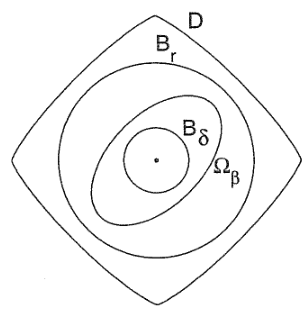
\includegraphics[scale=0.55]{figure/nonlinear/lyapunov-proof.png}
  \caption{定理 \ref{lyapunov} 的证明过程图示}
  \label{lyapunov_proof}
\end{figure}
\newpage
\begin{proof}
  对于$\varepsilon>0$,选取$r\in (0,\varepsilon]$使得\[B_r=\{x\in\R{}^n:\|x\|\le r\}\subset D\]
  令$\alpha=\min\limits_{\|x\|=r}V(x)$\footnote{有界闭集(紧集)上的连续函数必取得最值。},则由 \eqref{VPD} 得$\alpha>0$。取$\beta\in(0,\alpha)$并令\[\Omega_\beta=\{x\in B_r:V(x)\le \beta\}\]
  那么$\Omega_\beta$一定在$B_r$的内部(见图 \ref{lyapunov_proof})\footnote{可用反证法说明。假若$\Omega_\beta$不在$B_r$的内部,则必存在一点$p\in\Omega_\beta$处于$B_r$的边界上。此点处,$V(p)\ge\alpha>\beta$,然而根据$\Omega_\beta$的构成可知对于任意$x\in\Omega_\beta$均有$V(x)\le\beta$,这就产生了矛盾。}。
  若一状态轨线于$t=0$从$\Omega_\beta$中出发,则该轨线一定在所有时刻$t\ge 0$都留在$\Omega_\beta$内部,这是因为由式 \eqref{VdotNSD} 可得
  \[\dot{V}(x(t))\le 0\implies V(x(t))\le V(x(0))\le \beta,\forall t\ge 0\]
  由于$\Omega_\beta$是紧的(这是因为其封闭并以$B_r$为界),那么由定理 \ref{uniqsol},\eqref{freeofauto} 对于所有$t\ge 0$与所有初始状态$x(0)\in\Omega_\beta$均存在唯一解。由于$V(x)$是连续的,且$V(0)=0$,因此存在$\delta>0$使得\[\|x\|\le\delta\implies V(x)<\beta\]
  那么\[B_\delta\subset\Omega_\beta\subset B_r\]且\[x(0)\in B_\delta\implies x(0)\in\Omega_\beta\implies x(t)\in\Omega_\beta\implies x(t)\in B_r\]
  因此\[\|x(0)\|<\delta\implies \|x(t)\|<r\le\varepsilon,\forall t\ge 0\]
  这就说明平衡点$x=0$是稳定的。

  现在假设 \eqref{VdotND} 成立。为证明渐近稳定性,需证明$t\to\infty$时$x(t)\to 0$,也就是证明对于每个$a>0$,均存在一$T>0$使得$\|x(t)\|<a,\forall t>T$。类似上面论述可得对于每个$a>0$,均存在$b>0$使得$\Omega_b\subset B_a$。因此,只需证明$t\to\infty$时$V(x(t))\to 0$即可\footnote{取任意的$a>0$,那么其中总存在$\Omega_b\subset B_a$。若证明了$t\to\infty$时$V(x(t))\to 0$,那么对于任意$b>0$均存在$T$使得$V(x(t))<b,\forall t>T$,也即时间足够长时总有$x(t)\in\Omega_b$,也就是$x(t)\in B_a$,即$\|x(t)\|<a,\forall t>T$。}。
  因为$V(x(t))$单调递减且有下界$0$,因此\[V(x(t))\to c\ge 0,t\to\infty\]
  为证明$c=0$,用反证法。假设$c\ne 0$。由于$V(x)$的连续性,存在$d>0$使得$B_d\subset\Omega_c$。$V(x(t))\to c> 0$意味着对于所有$t\ge 0$,$x(t)$均在球$B_d$外。令$-\gamma=\max\limits_{d\le\|x\|\le r}\dot{V}(x)$(其存在性之缘由同脚注1)。由 \eqref{VdotND} 可得$-\gamma<0$。因此\[V(x(t))=V(x(0))+\int_{0}^{t}\dot{V}(x(\tau))\diff\tau\le V(x(0))-\gamma t\]
  当$t$足够大时,上式右侧将一定变为负值,这和$c>0$的假设矛盾。
\end{proof}

需要特别注意,上述定理仅是充分的。下面用一实例说明。上述定理的推广见下一节。
\enlargethispage{1em}
\begin{example}[利用Lyapunov稳定性定理判别单摆系统稳定性]\label{suff_lyapunov}
  考虑例 \ref{pendulum} 所示的单摆系统。假设其不带阻尼,则其状态方程改写为
  \begin{equation}\label{nodamp}
    \begin{aligned}
      \dot{x}_1&=x_2\\
      \dot{x}_2&=-a\sin x_1
    \end{aligned}
  \end{equation}
  其中$a=g/l>0$。$x=0$为其平衡点,下面研究其稳定性。

  类似例 \ref{pendulum},我们很自然想到,选取其物理意义上的能量函数作为候选Lyapunov函数(Lyapunov function candidate):
  \begin{align*}
    V&=\frac{1}{2}m(lx_2)^2+mgl(1-\cos x_1)\\
    &=ml^2\left(\frac{1}{2}x_2^2+a(1-\cos x_1)\right)
  \end{align*}
  因子$ml^2>0$,不影响$V$的符号,则不妨定义Lyapunov函数为\begin{equation}\label{pendulum_candidate}
  V(x)=\frac{1}{2}x_2^2+a(1-\cos x_1)
\end{equation}
容易看出$V(0)=0$且$V(x)>0,-\pi<x_1<\pi,x_1\ne 0$。求其对$t$的导数可得\begin{align*}
  \dot{V}&=x_2\dot{x}_2+a(\sin x_1)\dot{x}_1\\
  &=a(\sin x_1){x}_2+x_2(-a\sin x_1)=0
\end{align*}
因此原点是稳定的,并且不是渐近稳定的。系统无阻尼,则单摆会一直保持摆动,$x_2$不会趋于$0$,故此论断是合理的。

再考虑有阻尼情形。此时状态方程改写为
  \begin{equation}\label{damped}
    \begin{aligned}
      \dot{x}_1&=x_2\\
      \dot{x}_2&=-a\sin x_1-bx_2
    \end{aligned}
  \end{equation}
其中$b=k/m$。
选取Lyapunov函数如式 \eqref{pendulum_candidate},类似例 \ref{pendulum} 对$t$求导可得$\dot{V}=-bx_2^2\le 0$,
其为负半定,因此我们只能得出原点稳定的结论。然而,原点实际上是渐近稳定的——从物理意义上考虑,有阻尼意味着单摆的摆动幅度会衰减,直至$t\to\infty$时停在最低点($\theta=0,\dot{\theta}=0$)。

事实上,这并不是定理 \ref{lyapunov} 出了问题,而是我们构造的Lyapunov函数不够“好”。我们基于式 \eqref{pendulum_candidate} 进行改造。
将$\frac12x_2^2$换成更加一般的二次型的形式$\frac12x^\mathrm{T}Px$,其中$P$为正定矩阵。则
\begin{align*}
  V&=\frac{1}{2}x^\mathrm{T}Px+a(1-\cos x_1)\\
  &=\frac{1}{2}\begin{bmatrix}
  x_1&x_2
  \end{bmatrix}\begin{bmatrix}
    p_{11}&p_{12}\\p_{12}&p_{22}
    \end{bmatrix}\begin{bmatrix}
      x_1\\x_2
      \end{bmatrix}+a(1-\cos x_1)
\end{align*}
其中$p_{11}>0,p_{11}p_{22}-p_{12}^2>0$。求其对$t$的导数可得\begin{align*}
  \dot{V}&=2\times \frac{1}{2}\begin{bmatrix}
    x_1&x_2
    \end{bmatrix}\begin{bmatrix}
      p_{11}\dot{x}_1+p_{12}\dot{x}_2\\p_{12}\dot{x}_1+p_{22}\dot{x}_2
      \end{bmatrix}+a(\sin x_1)\dot{x}_1\\
    &=\left(p_{11}\dot{x}_1x_1+p_{12}\dot{x}_2x_1+p_{12}\dot{x}_1x_2+p_{22}\dot{x}_2x_2\right)
        +a(\sin x_1)\dot{x}_1\\
      &=p_{11}x_1x_2+p_{12}x_1(-a\sin x_1-bx_2)+p_{12}x_2^2+p_{22}x_2(-a\sin x_1-bx_2)
      +a(\sin x_1)x_2\\
    &=(p_{11}-bp_{12})x_1x_2-p_{12}ax_1\sin x_1-(p_{22}b-p_{12})x_2^2+(1-p_{22})a(\sin x_1)x_2
\end{align*}
观察到(除去系数)第一项不定,第二项为正(注意$x_1\in(-\pi,\pi)$),第三项为正,第四项不定。
则只要让第一、第四项前系数为0,第二、第三项前系数为负即可使其负定。
则\[p_{11}-bp_{12}=0,p_{12}>0,p_{22}b-p_{12}>0,p_{22}=1\]
进而$p_{12}<b$,不妨取为$\frac{b}{2}$,此时$p_{11}=\frac{b^2}{2}>0$,则$p_{11}p_{22}-p_{12}^2=\frac{b^2}{2}-\frac{b^2}{4}>0$,验证得$P$仍为正定。这样得到
\begin{align*}
  \dot{V}=-\frac{1}{2}abx_1\sin x_1-\frac{1}{2}bx_2^2
\end{align*}
可得仅在原点为$0$,其余各处取值均为负,因此其为负定,进而由定理 \ref{lyapunov} 可得原点是渐近稳定的。

本例说明,当我们构造出的Lyapunov函数不适用渐近稳定条件时,不一定表明原系统就非渐近稳定,即定理 \ref{lyapunov} 仅是充分的,通俗地说,它可用于判别一系统{\bf 是}稳定或渐近稳定,但一般无法用于判别一系统{\bf 不是}稳定或渐近稳定。
\end{example}
\begin{example}[局部渐近稳定]
  考虑如下非线性系统\[\begin{aligned}\dot{x}_1&=x_1(x_1^2+x_2^2-2)-4x_1x_2^2\\\dot{x}_2&=x_2(x_1^2+x_2^2-2)+4x_1^2x_2\end{aligned}\]
  原点为其平衡点。构造如下正定函数\[V=\frac{1}{2}(x_1^2+x_2^2)\]
  求其对时间的导数得\[\begin{aligned}
    \dot{V}& =x_{1}\dot{x}_{1}+x_{2}\dot{x}_{2} \\
    &=x_{1}[x_{1}(x_{1}^{2}+x_{2}^{2}-2)-4x_{1}x_{2}^{2}]+x_{2}[x_{2}(x_{1}^{2}+x_{2}^{2}-2)+4x_{1}^{2}x_{2}] \\
    &=(x_1^2+x_2^2)(x_1^2+x_2^2-2)
    \end{aligned}\]
  在球域$B_r=\{x:x_1^2+x_2^2<2\}$内,$\dot{V}$是负定的。

  那么,原点是局部渐近稳定的。
\end{example}
我们“贪心地”希望渐近稳定对于大范围的初始条件都成立,而不是仅像上面例子那样对局部成立。
从定理 \ref{lyapunov} 的证明中可看出,若所有$x\in\mathbb{R}^n$都能找到一有界集合$\Omega_c$以包含之,则定理对全局成立。
这不仅需要$V$的定义域$D=\mathbb{R}^n$,还需要保持$\Omega_c$有界。而这需要对$V$作出进一步的要求。
下面的例子见于前言中参考文献1的123页和文献2的65页。

\begin{example}[径向有界]
  考虑\[V(x)=\frac{x_1^2}{1+x_1^2}+x_2^2\]
  取定$x_2=0$,当$x_1\to\infty$时,该函数趋于$1$,即其对于$x_1$而言是有界的。绘出其等值线如下图。
\begin{center}
  % 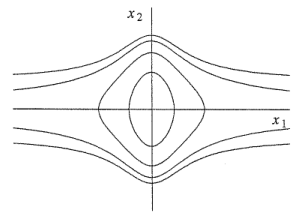
\includegraphics[scale=0.8]{figure/nonlinear/radially.png}
  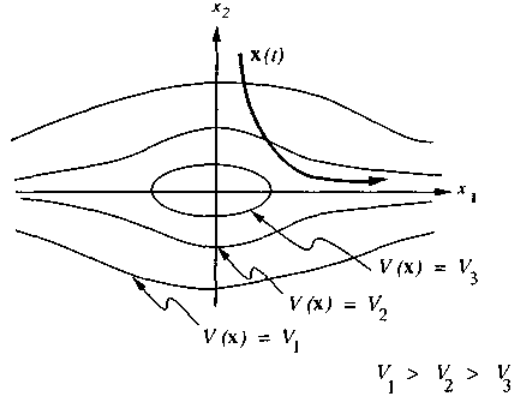
\includegraphics[scale=0.5]{figure/nonlinear/descent_but_unstable.png}
  \captionof{figure}{$V(x)=\frac{x_1^2}{1+x_1^2}+x_2^2$的等值线}
\end{center}
  对于较小的$c$,$V(x)=c$是闭合的,因此$\Omega_c$是有界的,如$\dot{V}<0$,则取一球域$B_r$包含之,即可同 \ref{lyapunov} 之证明找到球域$B_\delta$,使由其中出发的轨线都是渐近稳定的;
  随$c$增长,$V(x)=c$不再闭合,$\Omega_c$无界,则部分状态无法限制于有界$\Omega_c$,如图,从这类状态出发的轨线有可能沿着$V$下降的方向前往无穷远处!
\end{example}
可见,增加径向无界的要求,可能使定理 \ref{lyapunov} 对全局成立。
下述定理印证了这一想法。
\begin{theorem}[全局渐近稳定定理]
  设$V:\R{}^n\to\R$为连续可微函数,且满足
    \begin{itemize}[leftmargin=1em]
      \item $V(0)=0,V(x)>0,\forall x\in \R{}^n\backslash\{0\}$($V$为正定)
      \item $\dot{V}(x)< 0,\forall x\in \R{}^n$($\dot{V}$为负定)
      \item $\|x\|\to\infty\implies V(x)\to \infty$【$V$为径向无界(radially unbounded)\index{径向无界(radial unboundness)},或称为无限大】
    \end{itemize}
  则系统 \eqref{freeofauto} 的平衡点$x=0$是全局渐近稳定的。
\end{theorem}
\begin{proof}
  给定任意点$p\in\R{}^n$,令$c=V(p)$。径向无界条件意味着对任意$c>0$,都存在$r>0$使得$V(x)>c$对任意$\|x\|>r$成立。
  于是$\Omega_c\subset B_r$,则$\Omega_c$是有界的。剩余证明类似定理 \ref{lyapunov}。
\end{proof}
上述定理是下述定理的特例。
\begin{theorem}[Barbashin-Krasovskii定理]\index{Barbashin-Krasovskii定理}
  设$V:\R{}^n\to\R$为连续可微函数,且满足
    \begin{itemize}[leftmargin=1em]
      \item $V(0)=0,V(x)>0,\forall x\in \R{}^n\backslash\{0\}$($V$为正定)
      \item $\dot{V}(x)\le 0,\forall x\in \R{}^n$($\dot{V}$为负半定)
      \item 除零平衡点外,$\dot{V}=0$不包含系统任何整轨线
      \item $\|x\|\to\infty\implies V(x)\to \infty$($V$为径向无界,或称为无限大)
    \end{itemize}
  则系统 \eqref{freeofauto} 的平衡点$x=0$是全局稳定的。
\end{theorem}
具体证明过程略去,可参见前言中的参考文献3的2.3节。
上述定理是对定理 \ref{lyapunov} 的推广,放宽了导数负定的要求。

关于不稳定的判别,有下面定理。
\begin{theorem}[不稳定性判别定理]\label{unstable}
  对于系统 \eqref{freeofauto},若存在函数$V$,它在原点的任意邻域内是正定的,同时$\dot{V}$也是正定的,则系统的平衡点是不稳定的。
\end{theorem}